\documentclass{article}

% Language setting
% Replace `english' with e.g. `spanish' to change the document language
\usepackage[english]{babel}

% Set page size and margins
% Replace `letterpaper' with`a4paper' for UK/EU standard size
\usepackage[letterpaper,top=2cm,bottom=2cm,left=3cm,right=3cm,marginparwidth=1.75cm]{geometry}

% Useful packages
\usepackage{amsmath}
\usepackage{graphicx}
\usepackage{float}
\usepackage{subfigure}
\usepackage[colorlinks=true, allcolors=cyan]{hyperref}
\usepackage[title]{appendix}
\usepackage{caption}
\captionsetup[figure]{labelfont={bf}, name={Fig.}, labelsep=period}

\title{\textbf{\textsl{Dictyostelium}: Model System and Stress}}
\author{Group 9}
\date{}

\begin{document}
\maketitle

\begin{abstract}
\noindent Slime mold \textsl{Dictyostelium discoideum} lives in the soil in the form of uninucleate amoebae.
\end{abstract}

\section*{INTRODUCTION}
\textsl{Dictyostelium discoideum} has a unique developmental history. Uninucleate amoebae, or myxamoebae, is the form when cellular slime molds live in the soil as solitary. They prey on bacteria surrounding them and multiply.

\vspace{0.6em}\noindent
Slug migration and fruiting body formation arise as a result of responses of the pseudoplasmodia to environmental alteration \cite{newell_alternative_1969}.

\section*{MATERIALS AND METHODS}
\textbf{Fruiting in \textsl{Dictyostelium}} \textsl{Dictyostelium} was inoculated on the nutrient medium with prey bacteria to observe the growth of \textsl{Dictyostelium}. Firstly, 2-3 loopfuls of \textsl{E. coli} bacteria were spread in a strip in the center of two non-nutrient (NN) agar plates. (\textit{See materials on Appendix \ref{appendix:a}})

\section*{RESULTS}
\textbf{Fruiting in \textsl{Dictyostelium}} In the plate inoculated the \textsl{Dictyostelium}, \textsl{Dictyostelium} slug grew in the direction of the smeared \textsl{E. coli} (Fig.\ref{Fig.sub.1}). In the plate without treatment, there were no other bacteria, except \textsl{E. coli} (Fig.\ref{Fig.sub.2}).

\begin{figure}[H]
    \centering
    \subfigure[]{
    \label{Fig.sub.1}
    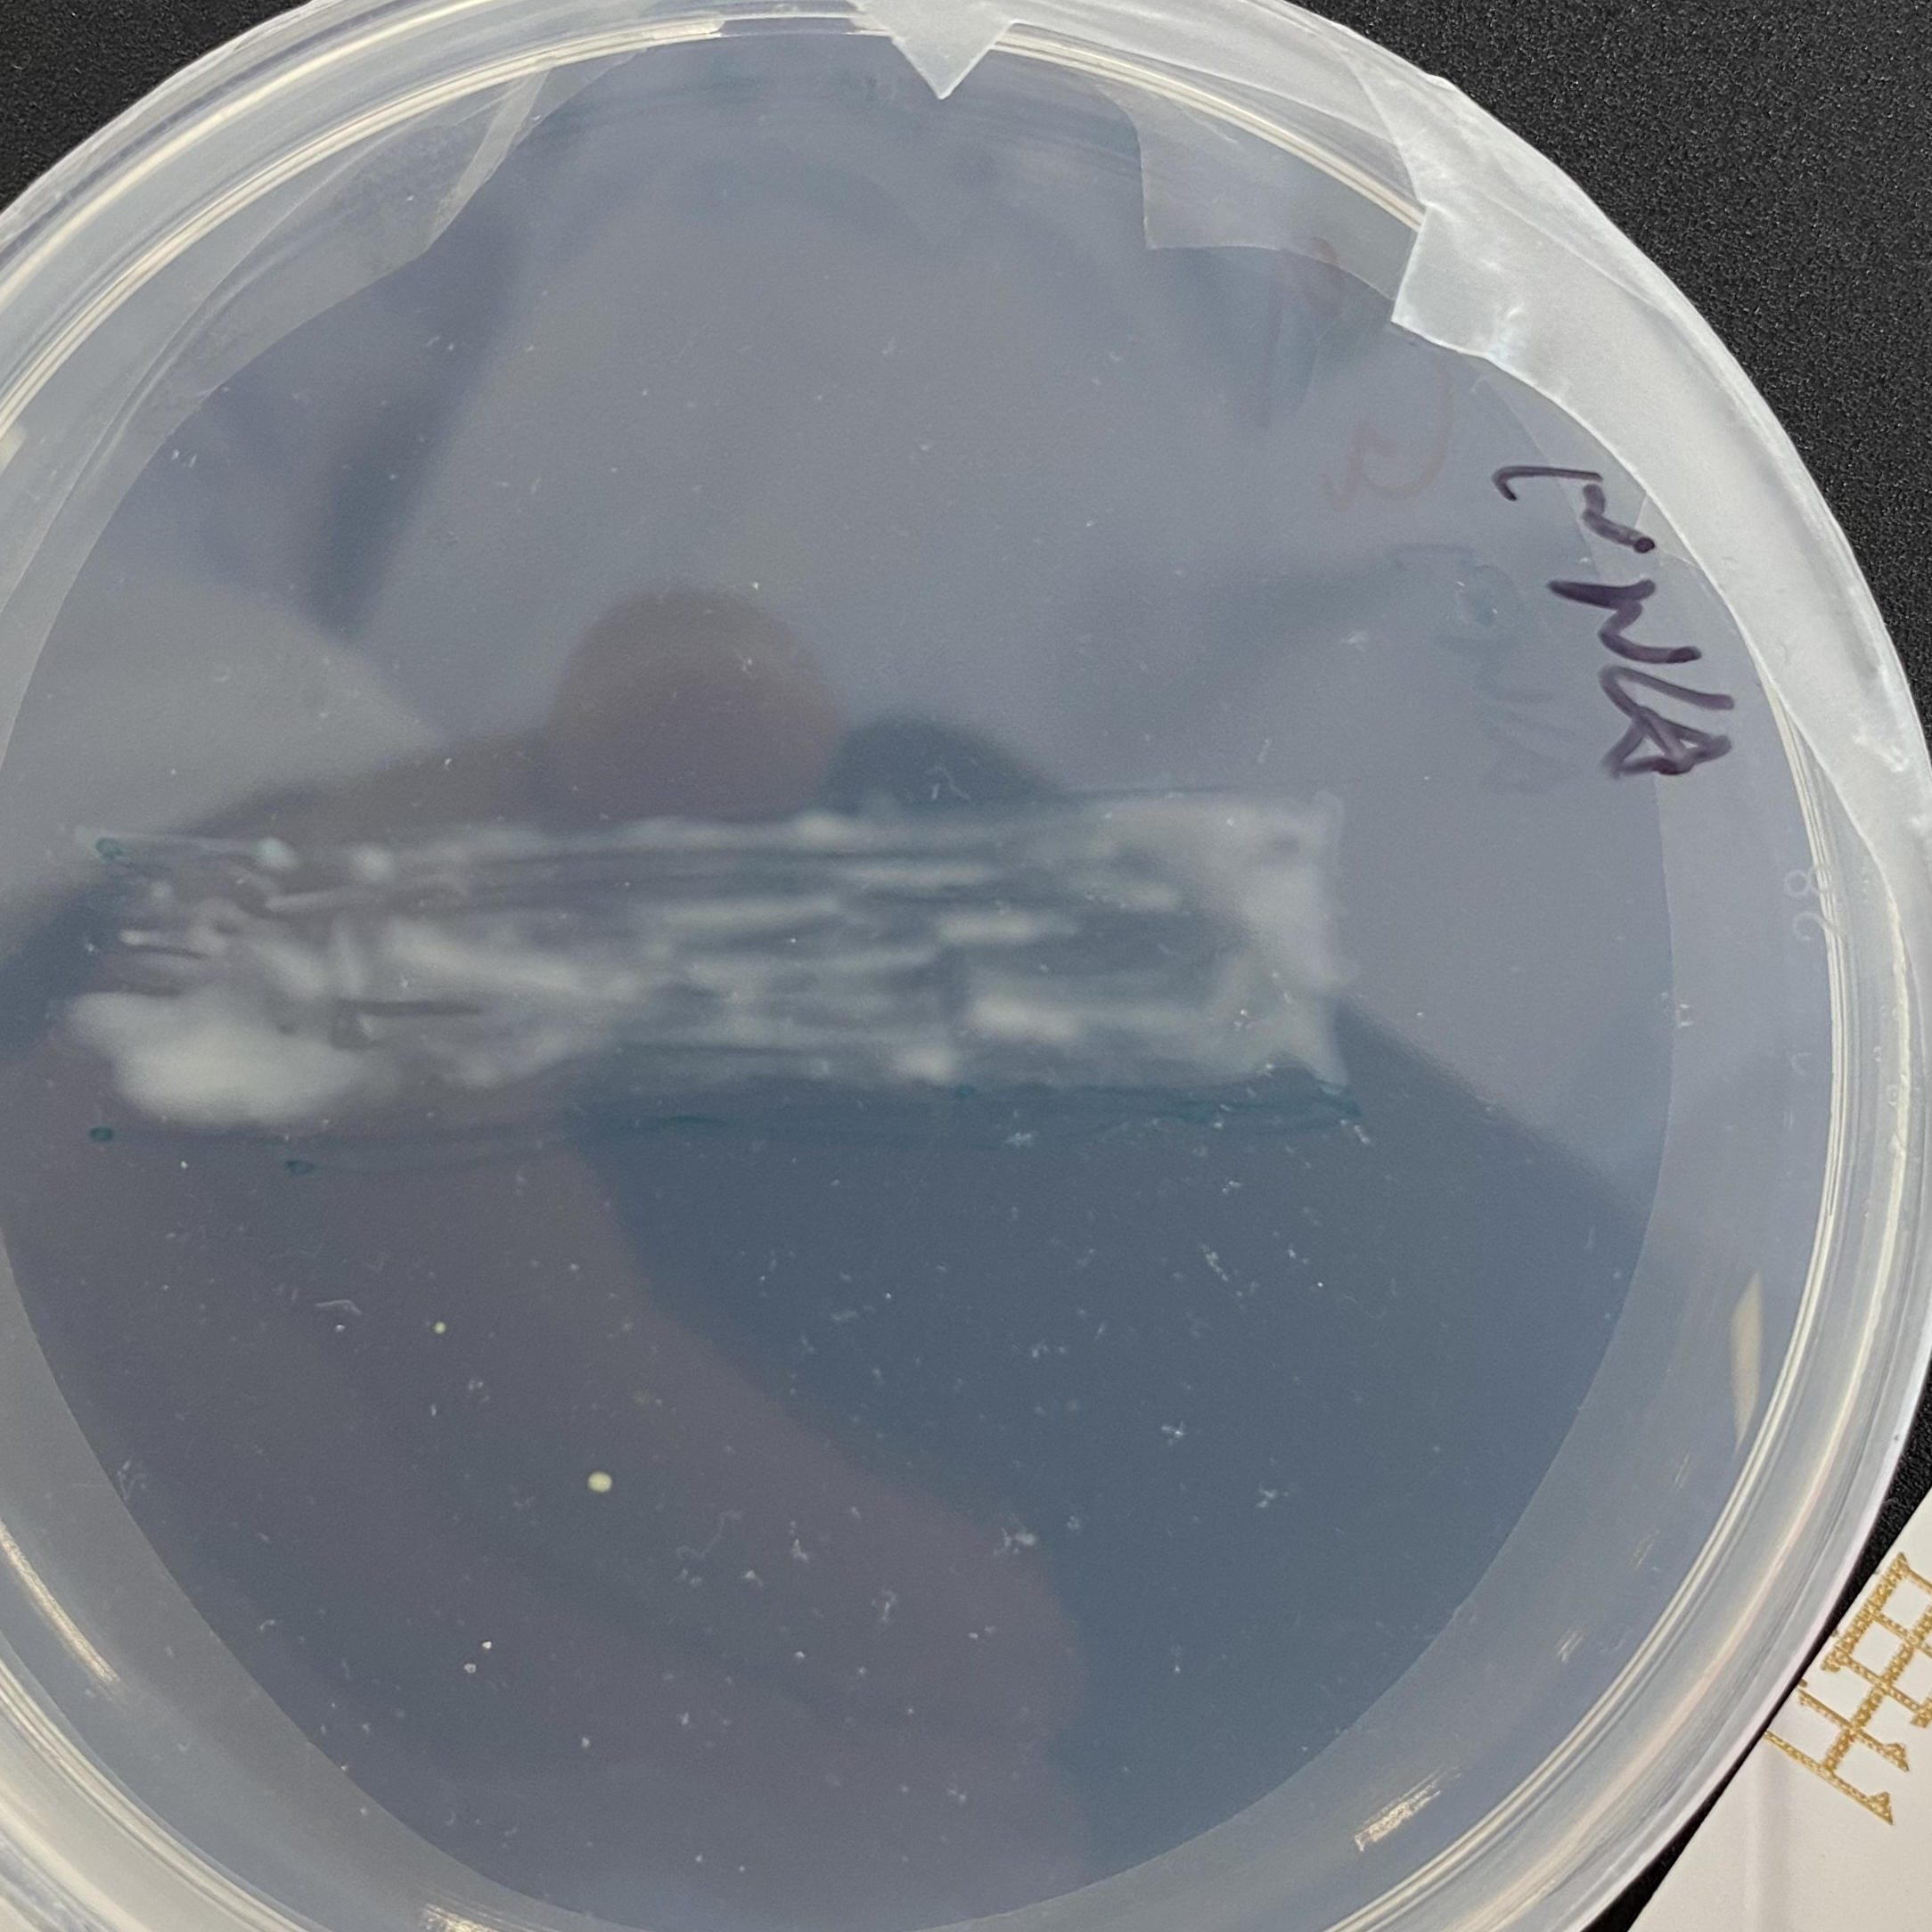
\includegraphics[width=0.26\textwidth, height = 0.25\textwidth]{figures/p1E.jpg}}
    \subfigure[]{
    \label{Fig.sub.2}
    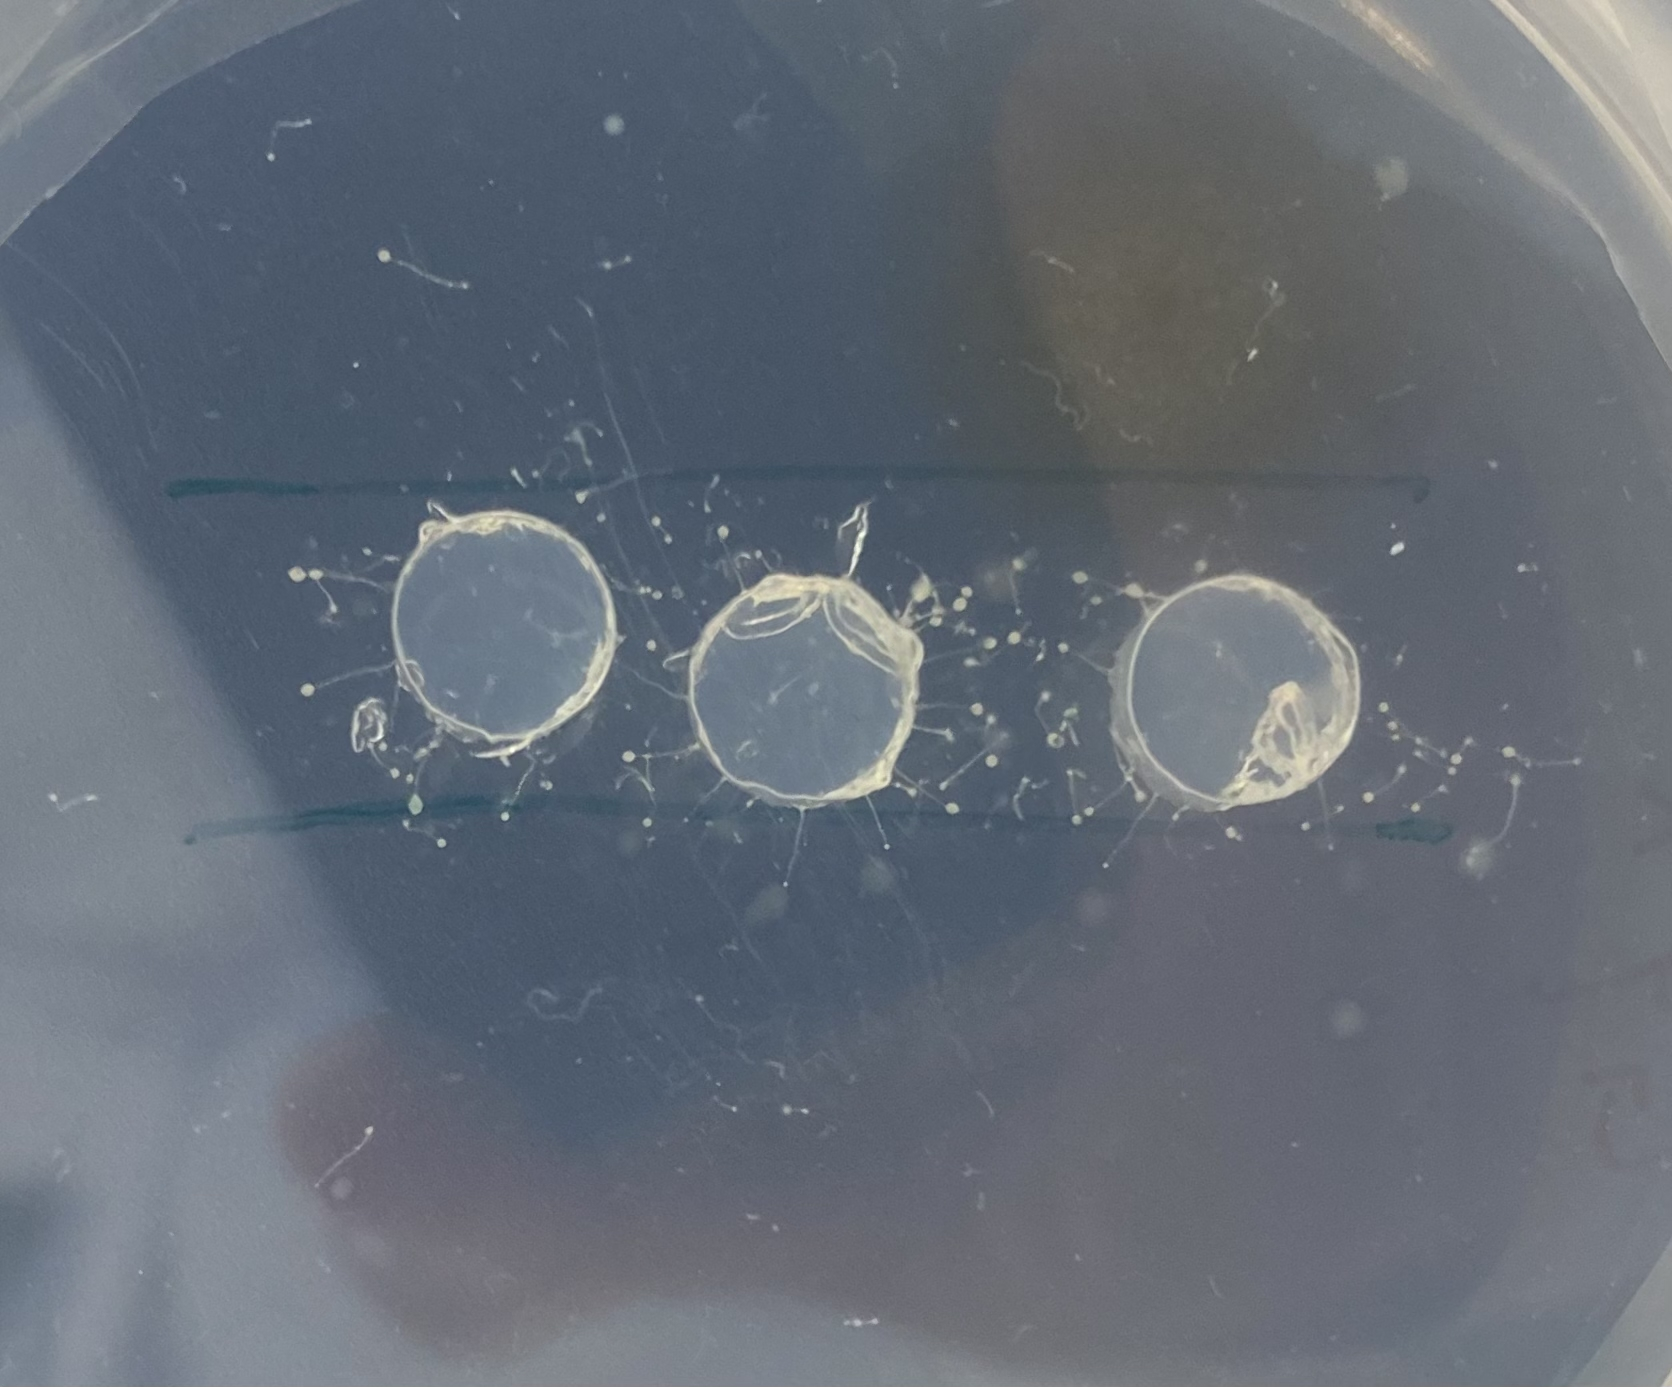
\includegraphics[width=0.26\textwidth, height = 0.25\textwidth]{figures/p1.jpg}}
    \caption{Fruiting in \textsl{Dictyostelium}. (a) Non-nutrition agar with \textsl{E.coli}. The white band is the \textsl{E.coli} bacteria smeared on the NNA. (b) Non-nutrition agar with \textsl{E.coli} and \textsl{Dictyostelium}. The three discs were cut from the \textsl{Dictyostelium} stock and inverted into the \textsl{E.coli} band.}
    \label{fig:my_label}
\end{figure}


\section*{DISCUSSION}
Cell differentiation and morphogenesis will happen in the growth of \textsl{Dictyostelium}, which is caused by gene expression and cell movement \cite{gross_developmental_1994}.

\section*{CONCLUSION}
Three experiments were conducted respectively to verify the importance of the environment, the phototaxis of \textsl{D. discoideum}, and the effect of sugars and peptone on \textsl{D. discoideum} fruiting. 

\bibliographystyle{unsrt}
\bibliography{Bib}

\clearpage
\begin{appendices}
\section{Materials in the practical}

\subsection{Fruiting in \textsl{Dictyostelium}}
\begin{itemize}
    \item [-] 1 Bunsen burner 
    \item [-] Toothpicks/blue tips 
    \item [-] 1 Mounted needle 
    \item [-] 1 Large loop 
    \item [-] 1 plate \textsl{E.coli} lawn grown on SM agar 
    \item [-] 2 plates non-nutrient agar (NNA) 
    \item [-] 1 plate \textsl{Dictyostelium} on steak of agar
\end{itemize}
\label{appendix:a}

\label{appendix:c}
\end{appendices}

\end{document}